\documentclass[11pt,a4paper]{report}
\usepackage[textwidth=37em,vmargin=30mm]{geometry}
\usepackage{calc,xunicode,amsmath,amssymb,paralist,enumitem,tabu,booktabs,datetime2,xeCJK,xeCJKfntef,listings}
\usepackage{tocloft,fancyhdr,tcolorbox,xcolor,graphicx,eso-pic,xltxtra,xelatexemoji}

\newcommand{\envyear}[0]{2025}
\newcommand{\envdatestr}[0]{2025-01-02}
\newcommand{\envfinaldir}[0]{webdb/2025/20250102/final}

\usepackage[hidelinks]{hyperref}
\hypersetup{
    colorlinks=false,
    pdfpagemode=FullScreen,
    pdftitle={Web Digest - \envdatestr}
}

\setlength{\cftbeforechapskip}{10pt}
\renewcommand{\cftchapfont}{\rmfamily\bfseries\large\raggedright}
\setlength{\cftbeforesecskip}{2pt}
\renewcommand{\cftsecfont}{\sffamily\small\raggedright}

\setdefaultleftmargin{2em}{2em}{1em}{1em}{1em}{1em}

\usepackage{xeCJK,xeCJKfntef}
\xeCJKsetup{PunctStyle=plain,RubberPunctSkip=false,CJKglue=\strut\hskip 0pt plus 0.1em minus 0.05em,CJKecglue=\strut\hskip 0.22em plus 0.2em}
\XeTeXlinebreaklocale "zh"
\XeTeXlinebreakskip = 0pt


\setmainfont{Brygada 1918}
\setromanfont{Brygada 1918}
\setsansfont{IBM Plex Sans}
\setmonofont{JetBrains Mono NL}
\setCJKmainfont{Noto Serif CJK SC}
\setCJKromanfont{Noto Serif CJK SC}
\setCJKsansfont{Noto Sans CJK SC}
\setCJKmonofont{Noto Sans CJK SC}

\setlength{\parindent}{0pt}
\setlength{\parskip}{8pt}
\linespread{1.15}

\lstset{
	basicstyle=\ttfamily\footnotesize,
	numbersep=5pt,
	backgroundcolor=\color{black!5},
	showspaces=false,
	showstringspaces=false,
	showtabs=false,
	tabsize=2,
	captionpos=b,
	breaklines=true,
	breakatwhitespace=true,
	breakautoindent=true,
	linewidth=\textwidth
}






\newcommand{\coverpic}[2]{
    % argv: itemurl, authorname
    Cover photo by #2~~(\href{#1}{#1})
}
\newcommand{\makeheader}[0]{
    \begin{titlepage}
        % \newgeometry{hmargin=15mm,tmargin=21mm,bmargin=12mm}
        \begin{center}
            
            \rmfamily\scshape
            \fontspec{BaskervilleF}
            \fontspec{Old Standard}
            \fontsize{59pt}{70pt}\selectfont
            WEB\hfill DIGEST
            
            \vfill
            % \vskip 30pt
            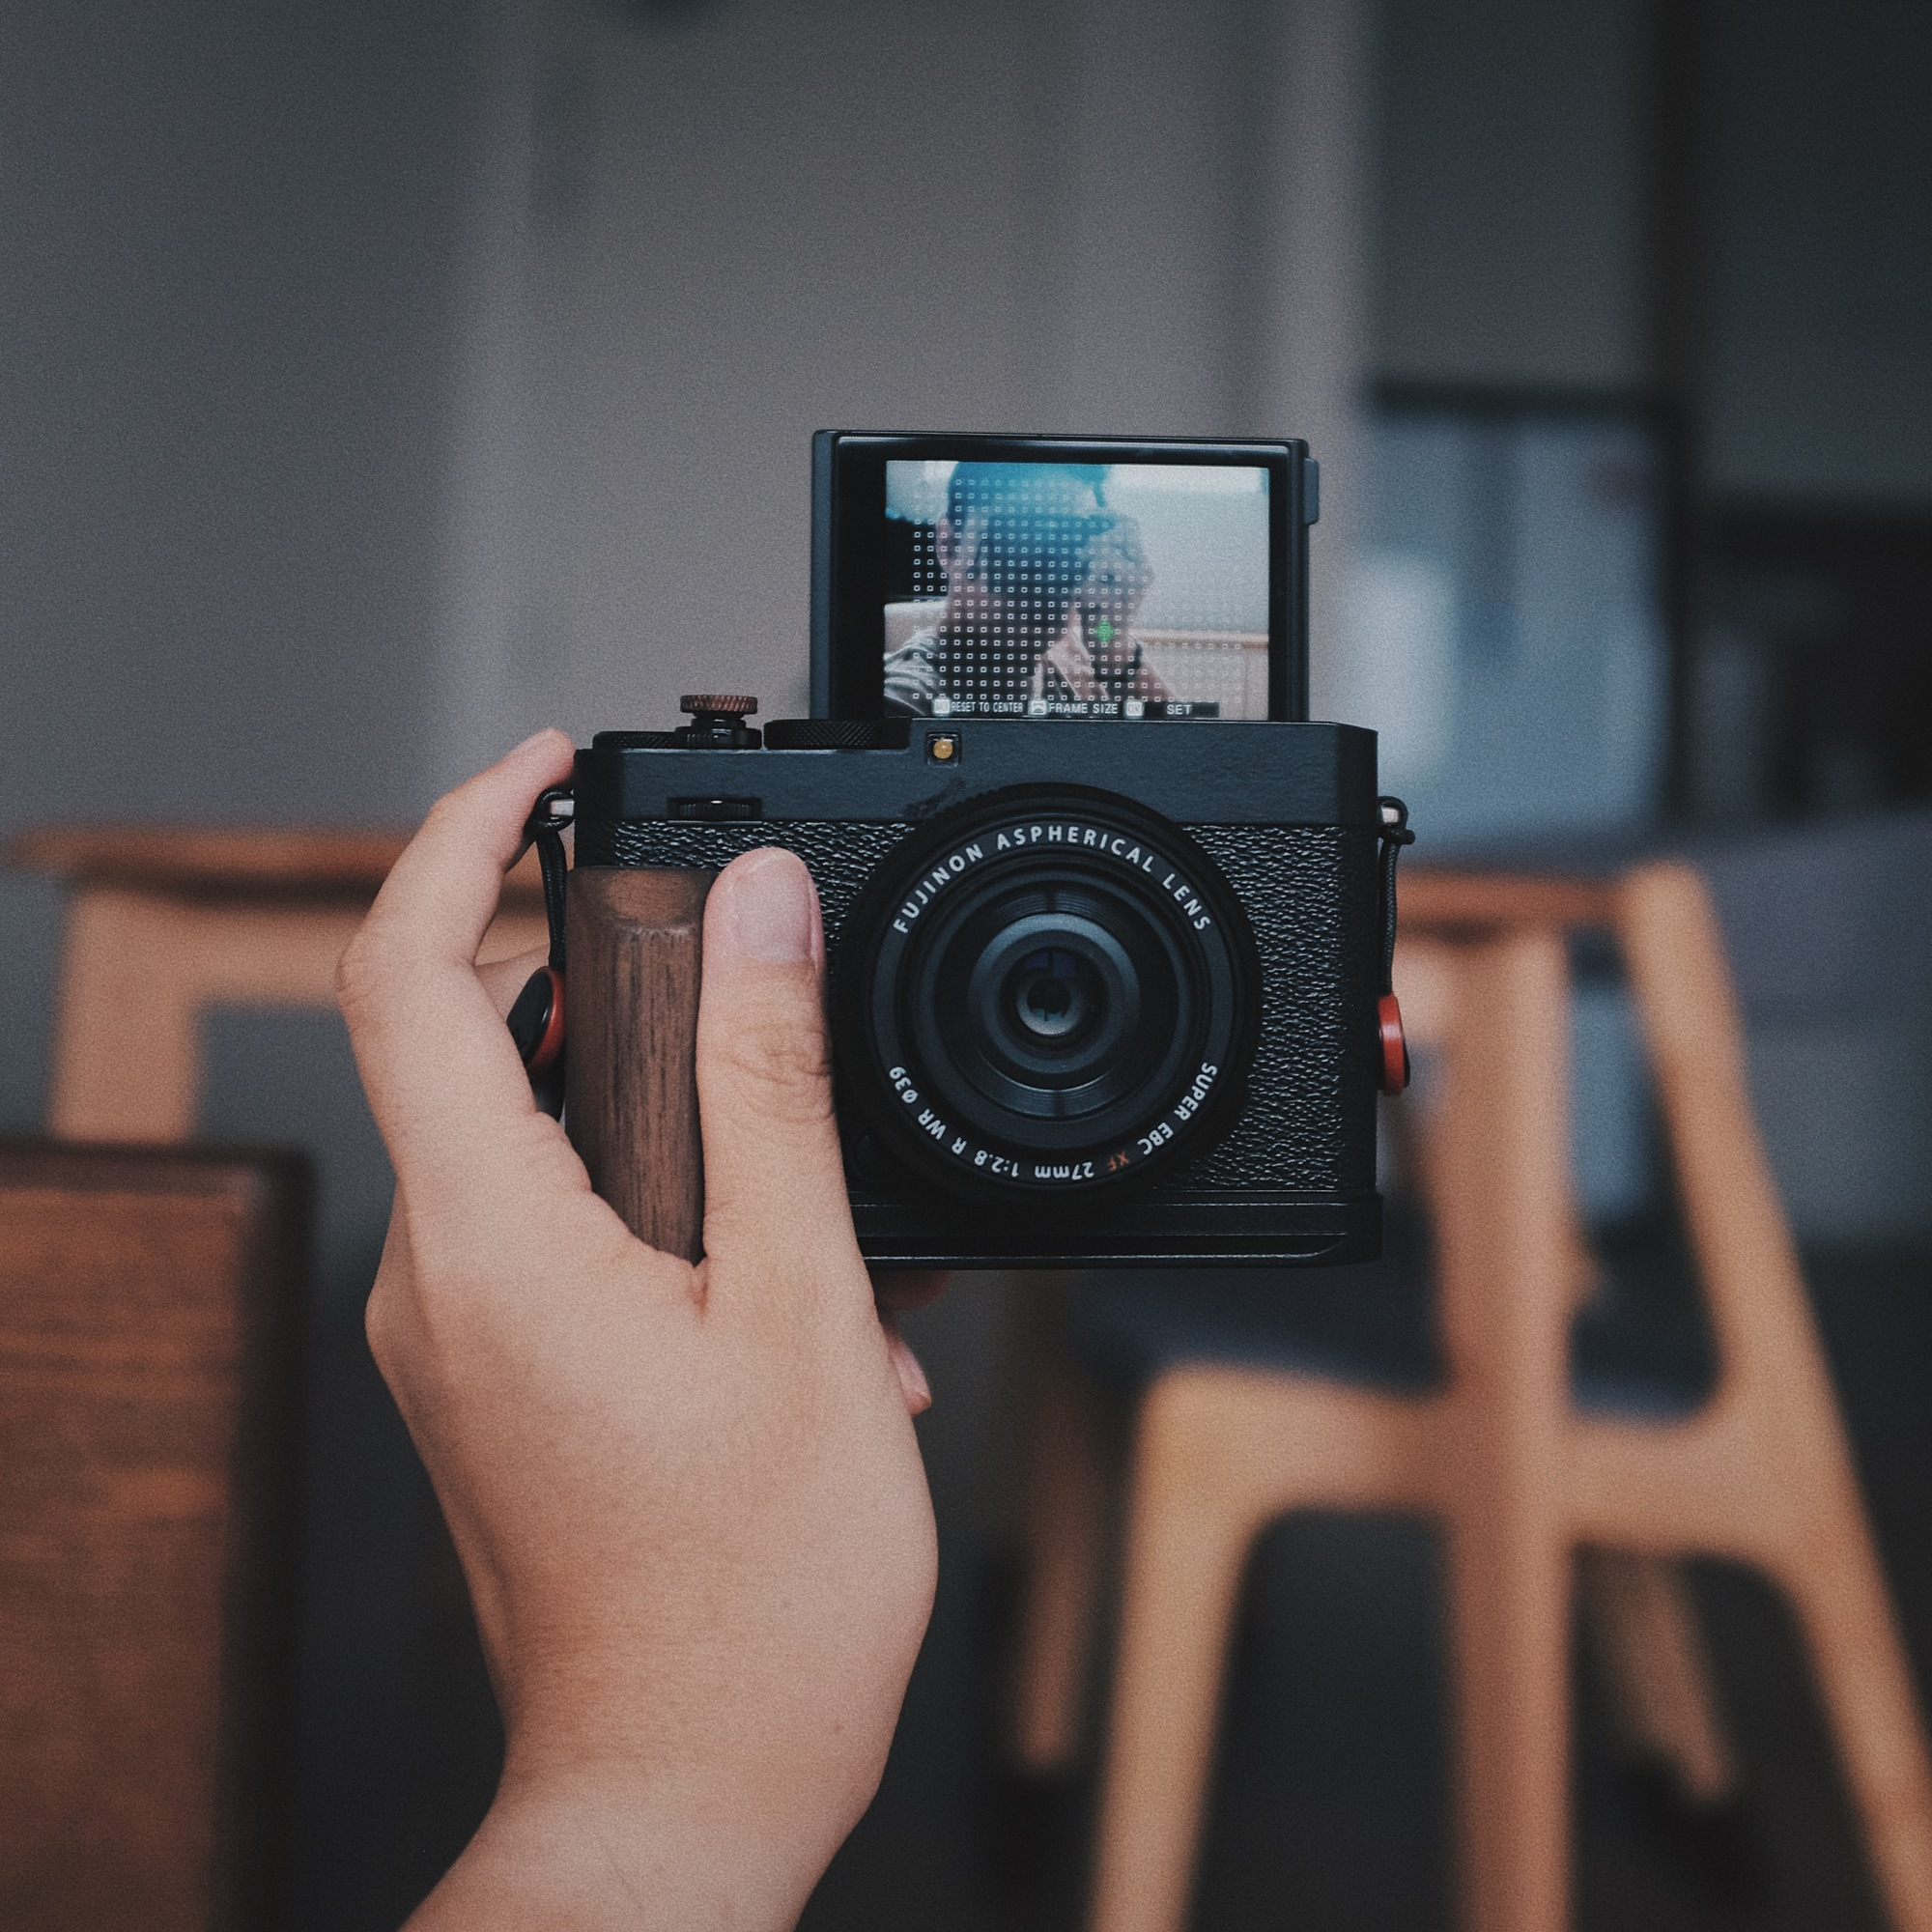
\includegraphics[width=\linewidth]{\envfinaldir/coverpic-prod.jpg}\par
            % \vskip 30pt
            \vfill

            \normalsize\rmfamily\scshape
            \copyright{} The Web Digest Project \hfill\large \envdatestr
        \end{center}
    \end{titlepage}
    % \restoregeometry
}
\newcommand{\simplehref}[1]{%
    \textcolor{blue!80!green}{\href{#1}{#1}}%
}
\renewcommand{\contentsname}{\center\Huge\sffamily\bfseries Contents\par\vskip 20pt}
\newcounter{ipartcounter}
\setcounter{ipartcounter}{0}
\newcommand{\ipart}[1]{
    % \vskip 20pt
    \clearpage
    \stepcounter{ipartcounter}
    \phantomsection
    \addcontentsline{toc}{chapter}{#1}
    % \begin{center}
    %     \Huge
    %     \sffamily\bfseries
    %     #1
    % \end{center}
    % \vskip 20pt plus 7pt
}
\newcounter{ichaptercounter}
\setcounter{ichaptercounter}{0}
\newcommand{\ichapter}[1]{
    % \vskip 20pt
    \clearpage
    \stepcounter{ichaptercounter}
    \phantomsection
    \addcontentsline{toc}{section}{\numberline{\arabic{ichaptercounter}}#1}
    \begin{center}
        \Huge
        \sffamily\bfseries
        #1
    \end{center}
    \vskip 20pt plus 7pt
}
\newcommand{\entrytitlefont}[1]{\subsection*{\raggedright\Large\sffamily\bfseries#1}}
\newcommand{\entryitemGeneric}[2]{
    % argv: title, url
    \parbox{\linewidth}{
        \entrytitlefont{#1}\par\vskip 5pt
        \footnotesize\ttfamily\mdseries
        \simplehref{#2}
    }\vskip 11pt plus 11pt minus 1pt
}
\newcommand{\entryitemGithub}[3]{
    % argv: title, url, desc
    \parbox{\linewidth}{
        \entrytitlefont{#1}\par\vskip 5pt
        \footnotesize\ttfamily\mdseries
        \simplehref{#2}\par\vskip 5pt
        \small\rmfamily\mdseries#3
    }\vskip 11pt plus 11pt minus 1pt
}
\newcommand{\entryitemAp}[3]{
    % argv: title, url, desc
    \parbox{\linewidth}{
        \entrytitlefont{#1}\par\vskip 5pt
        \footnotesize\ttfamily\mdseries
        \simplehref{#2}\par\vskip 5pt
        \small\rmfamily\mdseries#3
    }\vskip 11pt plus 11pt minus 1pt
}
\newcommand{\entryitemHackernews}[3]{
    % argv: title, hnurl, rawurl
    % \parbox{\linewidth}{
    %     \entrytitlefont{#1}\par\vskip 5pt
    %     \footnotesize\ttfamily\mdseries
    %     \simplehref{#3}\par
    %     \textcolor{black!50}{\href{#2}{#2}}
    % }\vskip 11pt plus 11pt minus 1pt
    \begin{minipage}{\linewidth}
            \entrytitlefont{#1}\par\vskip 5pt
            \footnotesize\ttfamily\mdseries
            \simplehref{#3}\par
            \textcolor{black!50}{\href{#2}{#2}}
    \end{minipage}\par\vskip 11pt plus 11pt minus 1pt
}







\begin{document}

\makeheader

\tableofcontents\clearpage




\ipart{Developers}
\ichapter{Hacker News}
\entryitemTwoLinks{Terence Tao: One of my papers got declined today}{https://news.ycombinator.com/item?id=42568399}{https://mathstodon.xyz/@tao/113721192051328193}

\entryitemTwoLinks{Welcome to the Public Domain in 2025}{https://news.ycombinator.com/item?id=42567280}{https://blog.archive.org/2025/01/01/welcome-to-the-public-domain-in-2025/}

\entryitemTwoLinks{Tesla replaces laid-off U.S. workers with foreigners using visas pushed by Musk}{https://news.ycombinator.com/item?id=42566784}{https://www.msn.com/en-ca/autos/electric-cars/tesla-replaces-laid-off-u-s-workers-with-foreigners-using-visas-pushed-by-musk-report/ar-AA1wILAQ}

\entryitemTwoLinks{Databases in 2024: A Year in Review}{https://news.ycombinator.com/item?id=42566192}{https://www.cs.cmu.edu/~pavlo/blog/2025/01/2024-databases-retrospective.html}

\entryitemTwoLinks{Ruby 3.4 Highlights}{https://news.ycombinator.com/item?id=42566141}{https://blog.sinjakli.co.uk/2025/01/01/ruby-3-4-highlights/}

\entryitemTwoLinks{DOOM CAPTCHA}{https://news.ycombinator.com/item?id=42566112}{https://doom-captcha.vercel.app/}

\entryitemTwoLinks{Show HN: API Parrot – Automatically Reverse Engineer HTTP APIs}{https://news.ycombinator.com/item?id=42565821}{https://apiparrot.com/}

\entryitemTwoLinks{30\% drop in O1-preview accuracy when Putnam problems are slightly variated}{https://news.ycombinator.com/item?id=42565606}{https://openreview.net/forum?id=YXnwlZe0yf\&noteId=yrsGpHd0Sf}

\entryitemTwoLinks{Books I Loved Reading in 2024}{https://news.ycombinator.com/item?id=42564687}{https://thoughts.wyounas.com/p/books-i-enjoyed-most-in-2024}

\entryitemTwoLinks{Cesium for Unreal – Bring the Real World to Unreal Engine}{https://news.ycombinator.com/item?id=42563845}{https://cesium.com/platform/cesium-for-unreal/}

\entryitemTwoLinks{Large Concept Models: Language modeling in a sentence representation space}{https://news.ycombinator.com/item?id=42563534}{https://github.com/facebookresearch/large\_concept\_model}

\entryitemTwoLinks{Static search trees: faster than binary search}{https://news.ycombinator.com/item?id=42562847}{https://curiouscoding.nl/posts/static-search-tree/}

\entryitemTwoLinks{Happy New Year 2025}{https://news.ycombinator.com/item?id=42562750}{https://news.ycombinator.com/item?id=42562750}

\entryitemTwoLinks{Déjà vu: Ghostly CVEs in my terminal title}{https://news.ycombinator.com/item?id=42562743}{https://dgl.cx/2024/12/ghostty-terminal-title}

\entryitemTwoLinks{FBI: Largest homemade explosives cache in agency history found in Virginia}{https://news.ycombinator.com/item?id=42562529}{https://thehill.com/national-security/5061535-virginia-man-arrested-explosives/}

\entryitemTwoLinks{Building Game Prototypes with LÖVE}{https://news.ycombinator.com/item?id=42562175}{https://healeycodes.com/building-game-prototypes-with-love}

\entryitemTwoLinks{Arnis: Generate cities in Minecraft from OpenStreetMap}{https://news.ycombinator.com/item?id=42561711}{https://github.com/louis-e/arnis}

\entryitemTwoLinks{Things we learned about LLMs in 2024}{https://news.ycombinator.com/item?id=42560558}{https://simonwillison.net/2024/Dec/31/llms-in-2024/}

\entryitemTwoLinks{Dinner for One: British comedy Germans have been laughing at for years (2018)}{https://news.ycombinator.com/item?id=42560171}{https://www.theguardian.com/tv-and-radio/2018/dec/30/dinner-for-one-german-television-new-years-eve}

\entryitemTwoLinks{The GTA III port for the Dreamcast has been released}{https://news.ycombinator.com/item?id=42559909}{https://gitlab.com/skmp/dca3-game}\ichapter{Phoronix}
\entryitemGeneric{\hskip 0pt{}X.Org Server Development Hit A Decade High For The Number Of Commits In 2024}{https://www.phoronix.com/news/X.Org-Server-2024-GitStats}

\entryitemGeneric{\hskip 0pt{}GCC Patches Posted For Half-Century Old ALGOL 68 Programming Language}{https://www.phoronix.com/news/GCC-ALGOL-68-Language-Front-End}

\entryitemGeneric{\hskip 0pt{}The Most Popular Linux \& Open-Source News Of 2024}{https://www.phoronix.com/news/Linux-Open-Source-News-2024}

\entryitemGeneric{\hskip 0pt{}Linux "hid-universal-pidff" Driver Proposed For Fixing More Quirky Devices}{https://www.phoronix.com/news/Linux-hid-universal-pidff}

\entryitemGeneric{\hskip 0pt{}Zlib-ng 2.2.3 Rings In The New Year With ~17.8\% Faster Inflate For AVX2}{https://www.phoronix.com/news/zlib-ng-2.2.3-Released}

\entryitemGeneric{\hskip 0pt{}RISC-V Made Nice Software Progress In 2024 While Interesting Hardware Still Rare}{https://www.phoronix.com/news/RISC-V-2024-Software-Progress}

\entryitemGeneric{\hskip 0pt{}Arch Linux Had A Great Year With Valve's Continued Backing, EndeavourOS \& CachyOS Boost}{https://www.phoronix.com/news/Arch-Linux-2024-Highlights}

\entryitemGeneric{\hskip 0pt{}The Linux Kernel Hit A Decade Low In 2024 For The Number Of New Commits Per Year}{https://www.phoronix.com/news/2024-Linux-Git-Stats}

\entryitemGeneric{\hskip 0pt{}Debian Installer Trixie Alpha 1 Brings RISC-V \& Drops i386 Installer}{https://www.phoronix.com/news/Debian-Installer-Trixie-Alpha-1}


\ipart{Developers~~~~(zh-Hans)}
\ichapter{Solidot}
\entryitemGeneric{\hskip 0pt{}diaspora*项目七成流量来自 AI 机器人}{https://www.solidot.org/story?sid=80209}

\entryitemGeneric{\hskip 0pt{}中端智能手机销量大幅下滑}{https://www.solidot.org/story?sid=80208}

\entryitemGeneric{\hskip 0pt{}《师父(SIFU )》在 Epic Games Store 限免 }{https://www.solidot.org/story?sid=80207}

\entryitemGeneric{\hskip 0pt{}天文学家利用韦伯望远镜发现烛龙螺旋星系}{https://www.solidot.org/story?sid=80206}

\entryitemGeneric{\hskip 0pt{}AI 数据中心影响美国居民的电力质量}{https://www.solidot.org/story?sid=80205}

\entryitemGeneric{\hskip 0pt{}中国计划 2025 年在戈壁滩建造钍基熔盐反应堆}{https://www.solidot.org/story?sid=80204}

\entryitemGeneric{\hskip 0pt{}黑客从地面劫持和修复 Beesat-1 立方体卫星}{https://www.solidot.org/story?sid=80203}

\entryitemGeneric{\hskip 0pt{}中国原油需求可能提前达到峰值}{https://www.solidot.org/story?sid=80202}

\entryitemGeneric{\hskip 0pt{}特斯拉用持 H-1B 签证的外国工人取代被裁的美国员工}{https://www.solidot.org/story?sid=80201}

\entryitemGeneric{\hskip 0pt{}小鼠实验显示间歇性禁食有助于逆转年龄相关的骨损伤}{https://www.solidot.org/story?sid=80200}

\entryitemGeneric{\hskip 0pt{}多家美国电信公司证实遭中国黑客组织入侵}{https://www.solidot.org/story?sid=80199}

\entryitemGeneric{\hskip 0pt{}研究称一支香烟会缩短 20 分钟寿命}{https://www.solidot.org/story?sid=80198}

\entryitemGeneric{\hskip 0pt{}美国财政部使用的远程管理软件遭中国黑客入侵}{https://www.solidot.org/story?sid=80197}

\entryitemGeneric{\hskip 0pt{}Mozilla 发布 Firefox AI 助手 Orbit}{https://www.solidot.org/story?sid=80196}

\entryitemGeneric{\hskip 0pt{}LineageOS 22.1 释出}{https://www.solidot.org/story?sid=80195}

\entryitemGeneric{\hskip 0pt{}烹调含硫蔬菜会促进反式脂肪酸的形成}{https://www.solidot.org/story?sid=80194}

\entryitemGeneric{\hskip 0pt{}欧盟通用充电器接口法律生效}{https://www.solidot.org/story?sid=80193}

\entryitemGeneric{\hskip 0pt{}生成式 AI 热杀死了 PC 和 Mac 的 8GB 版本}{https://www.solidot.org/story?sid=80192}

\entryitemGeneric{\hskip 0pt{}国际C语言混乱代码大赛庆祝 40 周年将重启}{https://www.solidot.org/story?sid=80191}

\entryitemGeneric{\hskip 0pt{}尼康新镜头能同时捕捉长焦和广角图像}{https://www.solidot.org/story?sid=80190}\ichapter{V2EX}
\entryitemGeneric{\hskip 0pt{}[问与答] 关于 b 站百大 up,是信息茧房还是 b 站推送有问题?}{https://www.v2ex.com/t/1101872}

\entryitemGeneric{\hskip 0pt{}[OpenAI] claude 3.5 sonnet (cursor 白嫖版) 依然是我用过最智能的 LLM}{https://www.v2ex.com/t/1101871}

\entryitemGeneric{\hskip 0pt{}[程序员] Flash 被放弃真的是因为安全问题吗?为什么 Adobe 不选择重写更安全的 Flash,而是直接放弃这么大的市场,很多老动画、游戏的官网都是 Flash 写的,十几年没人维护现在都打不开了。Ruffle 非常多效果都不支持模拟}{https://www.v2ex.com/t/1101870}

\entryitemGeneric{\hskip 0pt{}[酷工作] [远程] SaaS Rust 后端}{https://www.v2ex.com/t/1101869}

\entryitemGeneric{\hskip 0pt{}[生活] 感觉生死真的无常,新的一年好好珍惜眼前人}{https://www.v2ex.com/t/1101868}

\entryitemGeneric{\hskip 0pt{}[问与答] 域名被通信管理局要求注册商(易名)停止解析、禁止转移,强制转移有成功过的吗?}{https://www.v2ex.com/t/1101867}

\entryitemGeneric{\hskip 0pt{}[Apple] 个人目前比较满意的 Mac mini 鼠标}{https://www.v2ex.com/t/1101866}

\entryitemGeneric{\hskip 0pt{}[宽带症候群] 上海电信 229 套餐给 2.5G 口光猫吗}{https://www.v2ex.com/t/1101865}

\entryitemGeneric{\hskip 0pt{}[NAS] 谨慎用各种 NAS 系统提供的基于 Web 的文件管理}{https://www.v2ex.com/t/1101864}

\entryitemGeneric{\hskip 0pt{}[奇思妙想] 搞了个免折腾的 homeassistant}{https://www.v2ex.com/t/1101863}

\entryitemGeneric{\hskip 0pt{}[问与答] 只有 x86 苹果电脑如何编译出适合 m1m2 的 app}{https://www.v2ex.com/t/1101862}

\entryitemGeneric{\hskip 0pt{}[投资] 美股大佬请进,咨询一下定投 ETF 手续费问题}{https://www.v2ex.com/t/1101861}

\entryitemGeneric{\hskip 0pt{}[问与答] 大佬们, vue3 新人求教,就没有办法对 ref 包装的 obj 进行解构吗}{https://www.v2ex.com/t/1101860}

\entryitemGeneric{\hskip 0pt{}[随想] 某些国内企业赚得少,吃相还很难看}{https://www.v2ex.com/t/1101856}

\entryitemGeneric{\hskip 0pt{}[分享创造] [开源] 零成本语义搜索引擎(基于 Cloudflare 免费账号)}{https://www.v2ex.com/t/1101855}

\entryitemGeneric{\hskip 0pt{}[随想] 跨年晚会 最喜欢的是北京卫视}{https://www.v2ex.com/t/1101853}

\entryitemGeneric{\hskip 0pt{}[宽带症候群] 家用宽带主路由求推荐}{https://www.v2ex.com/t/1101851}

\entryitemGeneric{\hskip 0pt{}[分享创造] 用 AutoHotkey 动态切换 Windows 的电源设置,强化低频下的响应性能}{https://www.v2ex.com/t/1101850}

\entryitemGeneric{\hskip 0pt{}[问与答] 如果是个体户给网站申请支付宝支付的话能在 pc 端, 移动端,微信公众号里通用吗? 有知道的吗?多谢}{https://www.v2ex.com/t/1101849}

\entryitemGeneric{\hskip 0pt{}[问与答] 你小时候读过读者文摘吗}{https://www.v2ex.com/t/1101848}

\entryitemGeneric{\hskip 0pt{}[macOS] 48G MBP M4 性价比如何?}{https://www.v2ex.com/t/1101847}

\entryitemGeneric{\hskip 0pt{}[Notion] 为什么 notion 目录不会固定}{https://www.v2ex.com/t/1101845}

\entryitemGeneric{\hskip 0pt{}[问与答] 国内的手机早就用安卓 15 很久了,为什么三星还是安卓 14。}{https://www.v2ex.com/t/1101844}

\entryitemGeneric{\hskip 0pt{}[程序员] 发现小学生在学 GoC 语言}{https://www.v2ex.com/t/1101843}

\entryitemGeneric{\hskip 0pt{}[宽带症候群] 020 电信竟然把公网 ip 回收了}{https://www.v2ex.com/t/1101842}

\entryitemGeneric{\hskip 0pt{}[程序员] 预算 500 元,找人定制一个自动注册脚本}{https://www.v2ex.com/t/1101841}

\entryitemGeneric{\hskip 0pt{}[NAS] 硬盘坏了,都是哪里找修复方便快捷?}{https://www.v2ex.com/t/1101840}

\entryitemGeneric{\hskip 0pt{}[问与答] obsidian 的插件及配置可以在多端之间同步吗?}{https://www.v2ex.com/t/1101839}

\entryitemGeneric{\hskip 0pt{}[北京] 2024 回顾与 2025 的展望}{https://www.v2ex.com/t/1101838}

\entryitemGeneric{\hskip 0pt{}[问与答] 坐标上海本人于 2024 年 12 月 31 号接到裁员通知}{https://www.v2ex.com/t/1101837}

\entryitemGeneric{\hskip 0pt{}[NAS] 硬盘容量不够,除了买买买,还有没其他方案?}{https://www.v2ex.com/t/1101836}

\entryitemGeneric{\hskip 0pt{}[程序员] 2024,被裁后独立开发者的第一年,赚了多少钱}{https://www.v2ex.com/t/1101835}

\entryitemGeneric{\hskip 0pt{}[问与答] 你觉得照片和镜子中的自己哪个更帅?}{https://www.v2ex.com/t/1101833}

\entryitemGeneric{\hskip 0pt{}[问与答] 避坑:毛毛虫点读笔!}{https://www.v2ex.com/t/1101832}

\entryitemGeneric{\hskip 0pt{}[推广] 元旦 T 楼! 送 YouTube Premium + 京东 E 卡 300 元}{https://www.v2ex.com/t/1101831}

\entryitemGeneric{\hskip 0pt{}[分享创造] 2025 新年快乐!写了一个彩蛋送给大家!}{https://www.v2ex.com/t/1101830}

\entryitemGeneric{\hskip 0pt{}[VPS] 请问有人出搬瓦工 35 刀 DC9 吗,我来收一个,要求带原邮。}{https://www.v2ex.com/t/1101829}

\entryitemGeneric{\hskip 0pt{}[问与答] 请教:用 PCR532 复制公司门禁卡可以开门,但是小米手环 7Pro 没反应}{https://www.v2ex.com/t/1101828}

\entryitemGeneric{\hskip 0pt{}[宽带症候群] 上海联通 2025 新年优惠套餐合辑有新套餐}{https://www.v2ex.com/t/1101825}

\entryitemGeneric{\hskip 0pt{}[问与答] 请问 windsurf 可以回滚到前面的代码吗?它有自动保存每一个修改的版本吗?}{https://www.v2ex.com/t/1101823}

\entryitemGeneric{\hskip 0pt{}[投资] 看三年炒股赚存下 200 万有感,大家来分享一下理财观念和理财收益吧}{https://www.v2ex.com/t/1101821}

\entryitemGeneric{\hskip 0pt{}[宽带症候群] (0757)电信宽带突然被回收了公网 IP,现在各处都处在 NAT4 了,原来的 hub 型组网方式,请教如何同等实现?}{https://www.v2ex.com/t/1101820}

\entryitemGeneric{\hskip 0pt{}[机器学习] 模型部署的姿势}{https://www.v2ex.com/t/1101819}

\entryitemGeneric{\hskip 0pt{}[iPhone] 13mini 美版有靠谱途径吗}{https://www.v2ex.com/t/1101818}

\entryitemGeneric{\hskip 0pt{}[macOS] 如何使用别人分享的 Xcode 文件在 mac 上安装浏览器扩展}{https://www.v2ex.com/t/1101817}

\entryitemGeneric{\hskip 0pt{}[分享发现] 优酷 mac 客户端 在半夜观看视频, little snitch 突然提示有 优酷 mac 客户端在试图打开本机端口允许远程请求}{https://www.v2ex.com/t/1101816}

\entryitemGeneric{\hskip 0pt{}[生活] 2024,这一年来最深的七个感触}{https://www.v2ex.com/t/1101815}

\entryitemGeneric{\hskip 0pt{}[分享创造] Nrfr v1.0.0 免 Root 的 SIM 卡国家码修改工具,绕过 Tiktok 检测机制}{https://www.v2ex.com/t/1101812}

\entryitemGeneric{\hskip 0pt{}[生活] 新年第一天出了事故 我全责}{https://www.v2ex.com/t/1101811}

\entryitemGeneric{\hskip 0pt{}[Oracle] Oracle 安装步骤错了一步,体验不好,能否一键卸载:}{https://www.v2ex.com/t/1101809}


\ipart{Generic News}
\ichapter{AP News}
\entryitemWithDescription{\hskip 0pt{}Meghan, the Duchess of Sussex, returns to Instagram and posts a New Year's video}{https://apnews.com/article/06fc46f446f079aec0d90a2dcfe0713a}{}

\entryitemWithDescription{\hskip 0pt{}Blake Lively sues `It Ends With Us' director Justin Baldoni alleging harassment and smear campaign}{https://apnews.com/article/1aecaec0a51d8c45ea313a6f7dbff31b}{}

\entryitemWithDescription{\hskip 0pt{}Harry Chandler, Navy medic who survived Japan's attack on Pearl Harbor, dies at 103}{https://apnews.com/article/22e11aa91195ffd719ea9e4351322064}{}

\entryitemWithDescription{\hskip 0pt{}No. 5 Penn State bottles up Jeanty, beats No. 8 Boise State 31-14 in Fiesta Bowl}{https://apnews.com/article/986c53b8f96be37f68425651e5703566}{}

\entryitemWithDescription{\hskip 0pt{}PlayStations for guns are offered up in New Orleans}{https://apnews.com/article/eca1d2b4f7522053e639fc529203def3}{}

\entryitemWithDescription{\hskip 0pt{}Thief swipes \$13 million in jewels, handbags and cash from a London mansion}{https://apnews.com/article/5c4f3dcdb152154002935413a7e41909}{}

\entryitemWithDescription{\hskip 0pt{}Wimbledon finalist Gabriela Dabrowski reveals she played through 2024 after breast cancer diagnosis}{https://apnews.com/article/acc3d00d863b9285f191882e6509da0a}{}

\entryitemWithDescription{\hskip 0pt{}Wind, rain and the threat of floods play the spoiler for New Year's festivities in the UK}{https://apnews.com/article/287ecd42f65b601d774afaef8075e52b}{}

\entryitemWithDescription{\hskip 0pt{}Nearly all of Puerto Rico is without power on New Year's Eve}{https://apnews.com/article/b594dc464d469b812dc9b65c76cc16e9}{}

\entryitemWithDescription{\hskip 0pt{}Angelina Jolie and Brad Pitt reach divorce settlement after 8 years}{https://apnews.com/article/61ed3ce6da2258708ee04795a53aeebd}{}

\entryitemWithDescription{\hskip 0pt{}The month of December in pictures}{https://apnews.com/article/bd6899b2ce76a9a2d584c48a3aa0dfdc}{}

\entryitemWithDescription{\hskip 0pt{}It's called the `Winter Arc.' And for some, it's replacing New Year's resolutions}{https://apnews.com/article/69c6280f52b5b62ca3eda3a808f865fb}{}

\entryitemWithDescription{\hskip 0pt{}Brock Purdy's elbow was `on fire' after hit but he says his surgically repaired ligament is fine}{https://apnews.com/article/4184f13b1dc0025c70a9ae014055128f}{}\ichapter{联合早报}
\entryitemWithDescription{沈泽玮:台湾冲突阻遏法案只叫不咬?}{https://www.zaobao.com/news/china/story20240918-4758889}{美国众议院9月9日开启了长达一星期的``中国周'',共通过25项主要涉华法案。(法新社) 美国众议院在当地时间9月9日开启了长达一星期的``中国周'',在美国总统和国会选举举行之前,密集表决数十项与中国有关的法案,共通过25项主要涉华法案……}

\entryitemWithDescription{欧盟电动车关税投票倒计时 中国在分歧中寻支持}{https://www.zaobao.com/news/china/story20240917-4758953}{欧盟27个成员国将于9月25日就是否继续对进口自中国的电动汽车额外征税进行最后表决。图为上海港等待装运出口的电动汽车。(彭博社) 欧盟对中国电动汽车加征关税的投票进入倒计时,正在欧洲访问的中国商务部部长王文涛与欧盟多国政府高层就此进行协商,试图在立场分歧的成员国中争取到更多支持。 受访学者研判,欧盟对中国电动汽车加征关税不可避免,但具体的加税方式和幅度仍有一定弹性,这是王文涛此行与各国谈判的重点……}

\entryitemWithDescription{港府今年将举办逾400项国庆活动}{https://www.zaobao.com/news/china/story20240917-4759341}{再过十多天就是中国国庆75周年,香港天星小轮展示``国庆75周年''\,``三天免费搭小轮''等标语迎国庆。(中新社) 再过十多天就是中国国庆75周年,香港特区政府今年将举办逾400项庆祝活动,希望通过一连串活动庆祝国庆,并且弘扬爱国主义教育及刺激消费。 港府星期二(9月17日)召开记者会,介绍各项庆祝国庆活动和特别优惠,涉及出行及吃喝玩乐等领域……}

\entryitemWithDescription{美空军部长:中国大陆军演精密化 为入侵封锁台湾做准备}{https://www.zaobao.com/news/china/story20240917-4759407}{美国空军部长肯德尔星期一(9月16日)在空军暨太空军协会的一场大会上致辞,提到中国对印太地区日益增长的威胁。(取自美国国防部网站) (华盛顿综合讯)美国空军部长肯德尔指,中国大陆军演的规模越来越大,也更加精密化,这是在专门为入侵、封锁台湾做准备。他也称,中国对印太地区的威胁现在已存在……}

\entryitemWithDescription{批准潜在对台备件军售案后 美派巡逻机过航台海}{https://www.zaobao.com/news/china/story20240917-4758770}{台军士兵8月26日在屏东县枋山训练场进行实弹演习时,从M1167 TOW运载车上发射一枚美制TOW-2A线导反坦克导弹。(路透社) (华盛顿/台北/北京综合讯)在批准潜在对台备件军售案之后,美国派遣反潜巡逻机过航台湾海峡,中国人民解放军东部战区则组织战机跟监美机,并誓言``坚决捍卫国家主权''……}

\entryitemWithDescription{李家超:若香港驻美经贸办被关 受害的是美企}{https://www.zaobao.com/news/china/story20240917-4758797}{香港特首李家超星期一(9月17日)警告,如果美国通过法案,导致香港驻美经贸办关闭,受害的是美国企业。图为李家超9月11日在``一带一路''高峰论坛上致辞。(彭博社) (香港综合讯)香港特首李家超警告,如果美国通过法案,导致香港驻美经贸办关闭,受害的是美国企业。 美国众议院上周通过《香港经济贸易办事处认证法案》,如果参议院也表决通过并交由总统签署成法,香港三个驻美国的经贸办可能将被强制关闭……}

\entryitemWithDescription{美国指中国航空工业集团员工企图实施黑客攻击}{https://www.zaobao.com/news/china/story20240917-4757988}{(华盛顿综合讯)中国航空航天巨头中国航空工业集团一名员工被指试图对美国宇航局、美国军方和其他目标展开黑客攻击。 据彭博社报道,美国检察官布坎南星期一(9月16日)在起诉书中,指控中国航空工业集团39岁的工程师吴宋(音译,Song Wu)企图从美国宇航局、空军、陆军和海军,以及联邦航空管理局取得电脑软件和源代码……}

\entryitemWithDescription{【东谈西论】恒大账务造假 普华永道是共犯还是被拖累?}{https://www.zaobao.com/news/china/story20240917-4756452}{因涉及恒大地产审计项目的违法行为,普华永道中国9月13日被中国财政部和证监会处以4.41亿人民币罚款并被令停业六个月, 广州分所被撤销……}

\entryitemWithDescription{戴庆成:香港输入人才计划大检阅}{https://www.zaobao.com/news/china/story20240917-4744978}{香港于2022年底推出高端人才通行证计划。(法新社) 2019年香港反修例风波过后,数以十万计港人移居海外,令香港出现人才荒。港府为了解决这个问题,在过去几年积极引入``新血'',当中以高才通计划最受瞩目,社会上也不时热议其成效。 高才通全称为高端人才通行证计划,于2022年底推出,申请人年收入须达到250万港元(约42万新元)以上,或本科毕业于全球百强大学并满足一定工作年限等……}

\entryitemWithDescription{中美希望稳定双边关系 中小国家可​​​搭建桥梁}{https://www.zaobao.com/news/china/story20240917-4745091}{中美元首去年11月在旧金山会晤后,双方都希望稳定两国关系,我国巡回大使陈庆珠认为,如果中美两国都认为走向战争不符合它们的利益,那么中小国家就可以做点什么,为双方搭建桥梁。 陈庆珠星期一(9月16日)在李光耀公共政策学院的一场研讨会上说,中国与西方的关系面对诸多困难,有中国智库表示,希望新加坡能协助在中美之间建立更多对话,``因为新加坡受美国信任,也在中国有渠道''……}

\entryitemWithDescription{陈庆珠:世界经历了三次``中国冲击'' 中美的主导力之争将继续}{https://www.zaobao.com/news/china/story20240917-4744996}{李光耀公共政策学院``思想之节庆''的一场研讨会,讨论``历史终结时的中国冲击''。左起是我国巡回大使陈庆珠、通商中国主席李奕贤、李光耀公共政策学院国际关系助理教授何莉菁、李光耀公共政策学院院长柯成兴……}

\entryitemWithDescription{上海遭遇75年来最强台风 扰乱民众中秋假期出行}{https://www.zaobao.com/news/china/story20240916-4745224}{台风贝碧嘉星期一(9月16日)登陆上海,维护人员星期一下午在衡山路上处理倒伏的树木。 (新华社) 台风造成上海上万株数目倒伏或折断。图为一棵倒下的大树砸坏一旁的建筑。(法新社) 台风贝碧嘉登陆上海后,黄浦江苏州河口潮位上涨,乌云密布。(中新社) 中国上海市星期一(9月16日)遭遇75年来最强台风``贝碧嘉''登陆,也是上海有记录以来首次有强台风侵袭……}

\entryitemWithDescription{陆男频长驱偷渡台湾在测试边防实力?}{https://www.zaobao.com/news/china/story20240916-4745161}{中国大陆一名王姓男子在中秋节前夕,乘橡皮艇从浙江宁波抵达台湾新北市林口,主动打电话投案,海巡署人员前去接他上岸。(自由時報) 中国大陆一名王姓男子划橡皮艇于上星期六清晨偷渡到台湾,隔天被新北市地方法院裁定羁押禁见。这是6月以来第二起大陆人士偷渡至台湾,此间专家质疑是否为海防破口,并怀疑对岸是否在测试台湾的边防实力……}

\entryitemWithDescription{中美时隔八月举行国防部工作会晤}{https://www.zaobao.com/news/china/story20240916-4745025}{(北京/华盛顿综合讯)中美双方上周末举行国防部工作会晤;美国官员称,美国积极进行美中两军外交活动,不代表美国对有关中国议题的处理方式发生任何改变。 据中国国防部星期天(15日)晚上通报,北京香山论坛结束后,第18次中美国防部工作会晤上星期六至星期天(9月14日至15日)在北京举行……}

\entryitemWithDescription{中国高校今年拟增足球运动本科专业}{https://www.zaobao.com/news/china/story20240916-4744925}{(北京综合讯)为了培养足球专业人才,中国大专学府今年度拟新增足球运动本科专业,以具体落实中国足球改革。 综合人民网和《南方都市报》报道,中国教育部上星期五(9月13日)发布《2024年度普通高等学校本科专业申报材料公示》。根据公示统计,今年度拟新增专业535个,涉及353所高校,其中39所高校新增足球运动专业……}

\entryitemWithDescription{香港23条首案 港男因穿``光时''上衣被定罪}{https://www.zaobao.com/news/china/story20240916-4743439}{(香港综合讯)香港一名无业男子,今年6月因穿印有2019年反修例抗争口号的上衣而被捕。他星期一承认违反煽动意图罪,成为在《维护国家安全条例》(即《香港基本法》第23条)下被定罪的第一人。 综合港媒《星岛日报》和路透社报道,27岁无业男子诸启邦今年6月12日在石门港铁站附近,未能出示身份证供查阅被警方拘捕……}

\entryitemWithDescription{美国务院:中国释放被关押近20年美籍牧师}{https://www.zaobao.com/news/china/story20240916-4744614}{(华盛顿综合电)中国释放被关押近20年的美国籍牧师,显示北京在中美关系的关键时刻展现善意。 综合彭博社、法新社和路透社报道,美国国务院发言人星期天(9月15日)说:``我们欢迎林大卫(音译,David Lin)从中华人民共和国的监狱获释。他已回返美国,这是他近20年来首次与家人见面。'' 林大卫的女儿艾丽斯告诉美国政治新闻网Politico,她的父亲将抵达得克萨斯州的圣安东尼奥……}

\entryitemWithDescription{中国驻泰使馆:近期并未向湄公河下游泄洪}{https://www.zaobao.com/news/china/story20240916-4743917}{(北京讯)泰国西北部的湄公河因洪水泛滥而决堤,中国否认这是中方泄洪所致,并称近来已持续减少云南景洪水电站的出库流量,以助下游地区抗洪。 中国驻泰国大使馆星期日(9月15日)深夜在官方微信公众号发文说,当天又有媒体报道称中国正在向湄公河泄洪,经向中国主管部门核实,使馆再次澄清,为帮助下游地区应对洪灾,中方近来持续稳定和减少景洪水电站出库流量,不可能对下游地区抗洪救灾形成压力……}

\entryitemWithDescription{加入美国储存可靠度评估计划 台湾军方编列预算采购三类型导弹}{https://www.zaobao.com/news/china/story20240916-4743826}{(台北讯)据台媒报道,台湾军方持续向美国采购可简易操作的导弹,预计在2024年、2031年以前获得400枚``标枪''反装甲导弹、2485枚``刺针''人携式防空导弹……}

\entryitemWithDescription{韩咏红:中美分头追逐全球南方}{https://www.zaobao.com/news/china/story20240916-4730719}{9月5日,中国外长王毅(中)同中非合作论坛非方现任共同主席国塞内加尔外长法勒(左)、下任共同主席国刚果外长加科索(右),在北京共同会见中外记者并答问。(路透社) 进入气候宜人的9月,中国接连举行了两场受瞩目的国际会议,一是聚集非洲53国国家元首与政要的中非合作论坛,接着是周末刚闭幕的北京香山论坛。 两场活动的参与者不同,规模也有很大差距……}

\entryitemWithDescription{菲律宾船只撤离中菲争议海域后 将再派船接替}{https://www.zaobao.com/news/china/story20240915-4730494}{这张在9月15日拍摄,并由菲律宾海岸警卫队提供的照片显示,菲律宾海岸警卫队船马格巴努亚号抵达了菲国巴拉望岛的一个港口。菲律宾早前以发现填海活动为由,今年4月派出马格巴努亚号前往萨比纳礁。(法新社/菲律宾海岸警卫队) 菲律宾国家海事委员会星期天(9月15日)发声明称,该国海岸警卫队一艘巡逻舰已离开萨比纳礁争议海域……}

\entryitemWithDescription{台风贝碧嘉直击中国华东 多趟本地与沪杭间航班取消}{https://www.zaobao.com/news/china/story20240915-4730611}{9月15日在上海外滩滨江步道上,一名外籍游客的雨伞被大风吹起。台风贝碧嘉的中心当天下午5时位于上海市东偏南方大约435公里的东海海面上,中心附近最大风力有13级。(中新社) (上海/新加坡综合讯)台风贝碧嘉预计将为中国华东沿海地区带来狂风暴雨,多趟往返新加坡与上海和杭州的航班取消……}






\clearpage
\leavevmode\vfill
\footnotesize

Copyright \copyright{} 2023-2025 Neruthes and other contributors.

This document is published with CC BY-NC-ND 4.0 license.

The entries listed in this newsletter may be copyrighted by their respective creators.

This newsletter is generated by the Web Digest project.

The newsletters are also delivered via Telegram channel \CJKunderline{\href{https://t.me/webdigestchannel}{https://t.me/webdigestchannel}}.\\
RSS feed is available at \CJKunderline{\href{https://webdigest.pages.dev/rss.xml}{https://webdigest.pages.dev/rss.xml}}.

This newsletter is available in PDF at
\CJKunderline{\href{https://webdigest.pages.dev/}{https://webdigest.pages.dev/}}.

The source code being used to generate this newsletter is available at\\
\CJKunderline{\href{https://github.com/neruthes/webdigest}{https://github.com/neruthes/webdigest}}.

This newsletter is also available in
\CJKunderline{\href{http://webdigest.pages.dev/readhtml/\envyear/WebDigest-20250102.html}{HTML}} and
\CJKunderline{\href{https://github.com/neruthes/webdigest/blob/master/markdown/\envyear/WebDigest-20250102.md}{Markdown}}.


\coverpic{https://unsplash.com/photos/a-black-table-topped-with-snowflakes-and-tags-JrbbAPXTqVo}{Kelly Sikkema}


\end{document}
